\documentclass[12pt, a4paper]{article}
\usepackage[utf8]{inputenc}
\usepackage[T2A]{fontenc}
\usepackage{indentfirst, setspace}
\usepackage{tabularx, multirow}
\usepackage[normalem]{ulem}
\usepackage[style=russian]{csquotes}
\usepackage[english,russian]{babel}
\usepackage{hyperref}
\usepackage{ragged2e}
\usepackage{caption}
\usepackage{wrapfig}
\usepackage{amsmath}
\usepackage{tikz}
\makeatletter
\def\@biblabel#1{#1. }
\makeatother
\captionsetup{labelsep=endash}
\usepackage{listings}
\linespread{1.3}
\lstset{
  language=C++,
  basicstyle=\ttfamily\small,
  keywordstyle=\color{blue},
  breaklines=true,
  commentstyle=\color{green},
  stringstyle=\color{red},
  extendedchars=\true,
  showstringspaces=false,
  keepspaces=true,
}

\usepackage[left=2cm,right=2cm,
    top=2cm,bottom=2cm,bindingoffset=0cm]{geometry}\begin{document}
\begin{titlepage}
     \fontsize{12}{12}\selectfont

  {\centering

   \begin{bf}

    \begin{wrapfigure}{l}{10mm}
        
\includegraphics[width=17mm]{photo_2023-11-16 10.21.16.jpeg}
    \end{wrapfigure}


    \noindent Министерство науки и высшего образования Российской Федерации

    \noindent Федеральное государственное бюджетное образовательное учреждение высшего образования

    \noindent \enquote{Московский государственный технический университет

     \noindent имени Н.Э. Баумана

     \noindent (национальный исследовательский университет)}

    \noindent (МГТУ им. Н.Э. Баумана)

   \end{bf}
  }

  \vspace{0.4cm}

  {\setstretch{0.1}
   \noindent\rule{\textwidth}{1mm}
   \noindent\rule{\textwidth}{0.5mm}

  }

  \fontsize{14}{21}\selectfont

  \noindent\begin{tabularx}{\textwidth}{l >{\centering\arraybackslash}X}
   ФАКУЛЬТЕТ & \flqq Фундаментальные Науки\frqq \\ \cline{2-2}

   КАФЕДРА & ФН-12 \flqq Математическое моделирование\frqq \\ \cline{2-2}
  \end{tabularx}

  \vspace{1cm}


  \begin{center}
   \begin{bf}

    \fontsize{24}{36}\selectfont
    ОТЧЕТ

    \fontsize{20}{30}\selectfont
    ПО ЛАБОРАТОРНОЙ РАБОТЕ НА ТЕМУ:

    Расстояние Левенштейна

   \end{bf}
  \end{center}

  \fontsize{14}{21}\selectfont
  \vspace{5cm}


  \noindent\begin{tabularx}{\textwidth}{ X >{\centering}p{4cm} p{1cm} c }
   Студент: & & & Мациевский И. М. \\ \cline{2-2} \cline{4-4}
   & \fontsize{10}{15}\selectfont дата, подпись & & \fontsize{10}{15}\selectfont Ф.И.О. \\
   Преподаватель: & & & Строганов Ю. В.\\ \cline{2-2} \cline{4-4}
   & \fontsize{10}{15}\selectfont дата, подпись & & \fontsize{10}{15}\selectfont Ф.И.О.
   \end{tabularx}

  \vspace{\fill}

  \begin{center}
   \it{Москва}, 2023
  \end{center}

  \thispagestyle{empty}
\end{titlepage}\newpage
\tableofcontents
\newpage
\section{Введение}
\subsection{Цель:}
Реализовать различные методы поиска расстояния
Левенштейна и  Дамерау-Левенштейна, сравнить их
эффективность
\textbf{Цель лабораторной работы}: провести сравнительный анализ алгоритмов поиска редакционных расстояний.

Для достижения поставленной цели требуется решить следующие \textbf{задачи}.
\begin{enumerate}
	\item Описать расстояния Левенштейна и Дамерау-Левенштейна.
	\item Разработать алгоритмы вычисления редакционных расстояний, согласно варианту.
	\item Реализовать разработанные алгоритмы.
	\item Выполнить тестирование реализации разработанных алгоритмов.
	\item Разработать программное обеспечение с двумя режимами работы --- режимом расчёта расстояний для введённых пользователем двух строк произвольной длины и режимом массированного замера процессорного времени для автоматически сгенерированных строк заданной длины.
	\item Провести сравнение временной эффективности реализации разработанных алгоритмов, проведя замеры процессорного времени их выполнения в зависимости от линейного размера строк одинаковой длины.
	\item Выполнить оценку емкостной эффективности разработанных алгоритмов в зависимости от линейных размеров строк (для рекурсивных алгоритмов дать оценку пиковой затрачиваемой памяти)
\end{enumerate}
Согласно варианту, требуется разработать следующие три алгоритма.
\begin{enumerate}
\item Нерекурсивный матричный алгоритм поиска 
расстояния Левенштейна;
\item Рекурсивный алгоритм поиска расстояния
Левенштейна без кэша;
\item Нерекурсивный алгоритм поиска расстояния
 Дамерау-Левенштейна на основе трех строк 
 матрицы.
\end{enumerate}
\newpage
\section{Аналитическая чаcть}
\subsection{Расстояние Левенштейна\\
Расстояние  Дамерау-Левенштейна}
\subsubsection{Определение}
Расстояние Левенштейна, или редакционное расстояние 
-- мера сходства между двумя строками. Численно 
равно количеству односимвольных 
преобразований(удаления,вставки или замены), 
необходимых для превращения одной строки в другую.

В случае расстояния  Дамерау-Левенштейна к 
односимвольным преобразованиям добавляется операция
перестановки двух соседних элементов
\subsubsection{Применение}
Алгоритмы поиска расстояний Левенштейна и
Дамерау-Левенштейна широко используются на
практике. Например, в биоинформатике для сравнения
ДНК, в интернет поисковиках и редакторских
программах, т.к. было доказано, что большинство
человеческих ошибок при наборе текста составляют 
перестановки соседних символов, пропуск символа,
добавление нового символа, и ошибка в символе.
 \subsubsection{Описание алгоритмов}
 Опишем алгоритм поиска расстояния Левенштейна,
 алгоритм поиска расстояния 
 Дамерау-Левенштейна будет во многом похож,
 поэтому описывать подробно и его мы не будем.\\
 Пусть $S_{1}$ и $S_{2}$ - строки длины х и у,
 расстояние между которыми нам нужно найти. Тогда
 расстояние d($S_{1}$, $S_{2}$)=D(x, y) можно найти
 по формуле:
 \begin{equation*}
D(i, j) = 
 \begin{cases}
   0 &\text{i = 0, j = 0}\\
   i &\text{j = 0, i > 0}\\
   j &\text{i = 0, j > 0}\\
   $min(D(i, j-1) + 1, D(i-1, j) + 1, D(i-1, 
   j-1) + f($S_{1}
   [i]$, $S_{2}$[j])$ &\text{i > 0, j > 0}\\
 \end{cases}
\end{equation*}
где f(a, b) = 0, если a=b, иначе равна 1, D(i, j) - 
расстояние между префиксами строк: первыми i
 символами строки $S_{1}$
 и первыми j
 символами строки $S_{2}$.\\
Чтобы найти формулу для расстояния  
Дамерау-Левенштейна, достаточно в формулу,
описанную выше, добавить случай перестановки
элементов:
\begin{equation*}
D(i, j) = 
 \begin{cases}
   min(A,D(i-2,j-2)+1) &\text{i>1, j>1, $S_{1}$
   [i]=$S_{2}$[j-1], $S_{1}$[i-1]=$S_{2}$[j]}\\ 
   A &\text{во всех остальных случаях}
 \end{cases}
\end{equation*}
\begin{equation*}
A = 
 \begin{cases}
   0 &\text{i = 0, j = 0}\\
   i &\text{j = 0, i > 0}\\
   j &\text{i = 0, j > 0}\\
   D(i-1,j-1) &\text{$S_{1}$[i]=$S_{2}$[j]}\\
   $min(D(i, j-1), D(i-1, j), D(i-1, j-1)+f($S_{1}$
   [i], $S_{2}$[j])$ &\text{i > 0, j > 0}\\
 \end{cases}
\end{equation*}
\subsection{Методы реализации}
Поиск этих расстояний можно реализовать разными 
способами, рассмотрим несколько из них:
\subsubsection{Рекурсивный}
В данной реализации нет ничего сложного, она 
заключается в обычном применении рекуррентной 
формулы сверху.\\
Рекурсия может быть очень 
долгой, поэтому можно ускорить данный алгоритм с 
использованием кэширование. Результат каждого поиска 
D(i,j) надо запомнить и при следующем вызове 
функции уже не придется еще раз считать это 
значение.
\subsubsection{Матричный}
Расстояние Левенштейна( Дамерау-Левенштейна) 
можно найти и без использования рекурсии.\\
Для этого необходимо составить матрицу D, в которой 
каждый элемент можно будет вычислить по рекуррентной 
формуле. Сначала вычисляется первая строка, затем первый 
столбец, по формуле понятно, что далее можно искать 
все элементы матрицы по строкам(начиная с первой и 
до последней).\\
В этой реализации тоже есть проблема - она
неэффективно использует память, если алгоритм 
запускается для строк длины $n$, матрица будет
размера $n^2$, но у этой проблемы есть решение, 
рассмотрим два случая: для расстояния Левештейна 
и расстояния  Дамерау-Левенштейна.
\paragraph{Расстояние Левенштейна, две строки.}
По формуле видно, что для поиска элемента матрицы 
D(i,j), нам нужна строка, в которой находится 
данный элемент и предыдущая строка, их мы и 
будем хранить, на больших строках это 
существенно уменьшит затраты памяти.
\paragraph{Расстояние  Дамерау-Левенштейна, три 
строки.}
Аналогично прошлому случае по формуле можно увидеть, 
что для поиска элемента матрицы нужно всего лишь 
две предыдущие и текущая строка, поэтому в этом 
случае тоже можно хранить только их.
\newpage
\section{Конструкторская часть}
\subsection{Нерекурсивный поиск расстояния 
Левенштейна с использованием матрицы}
\begin{enumerate}
	\item Создать матрицу $ans$ размером $(l1+1) 
	\times (l2+1)$, где $l1$ ~--~ длина первой 
	строки, а $l2$ ~--~ длина второй строки. 
	Заполнить первую строку значениями от 0 до $l1$ 
	(включительно), а первый столбец значениями от 0 
	до $l2$ (включительно);
	\item Завести два счетчика $i$ и $j$ по 
	элементам строк, пройти по каждой ячейке, начиная 
	с (1,1) по следующему правилу: если элементы 
	строк, на которые указывают счетчики равны, то в 
	ячейку $ans[i][j]$ записать минимум из трех 
	значений: значение ячейки сверху + 1, значение 
	ячейки слева + 1 и значение ячейки диагонально 
	сверху слева, иначе в ячейку $ans[i][j]$ записать 
	минимум из трех значений: значение ячейки сверху 
	+ 1, значение ячейки слева + 1 и значение ячейки
	диагонально сверху слева + 1;
	\item Итоговое редакционное расстояние будет в ячейке $ans[l1][l2]$.
\end{enumerate}
\subsection{Поиск расстояния  Дамерау-Левенштейна с 
  сохранением трех строк матрицы}   
\begin{enumerate}
  \item Инициализировать $second\_row$ числами от 1 
  до $l2$ -- предыдущая строка матрицы; 
  инициализируем $first\_row$, $first\_row[0]=1$ -- 
  текущая строка матрицы,  $third\_row$ -- следующая 
  строка матрицы;
  \item Вычисление значения элементов $first\_row[i]$ 
  по формуле: $first\_row[i] = min(second\_row[i] + 1, 
  first\_row[i-1] + 1, second\_row[i-1] + num)$, где 
  $num$ равен 0, если символы в позициях $i-1 $ и 
  $j-1$ в обоих строках равны, и равен 1 в противном 
  случае;
  \item Проверка на возможность использования 
  операции перестановки двух символов, стоящих рядом 
  друг с другом:
  Если $i > 1$ и $j > 1$, и символы в позициях $i-1$ 
  и $j-2$, $i-2$ и $j-1$ равны и если $first\_row[i] > 
  second\_row[i-1] + 1$ и $first\_row[i] > 
  first\_row[i-1] + 1$, то $first\_row[i] =
  second\_row[i-1] + 1$;
  \item Обновление prevRow, curRow и nextRow для 
  следующей итерации: $second\_row = first\_row$, 
  $first\_row = third\_row$. Создание новой строки для 
  $third\_row$, заполненной значениями начиная с $i + 
  1$, где $i$ - индекс символа во второй строке;
  \item Повторение шагов 2-4 для всех символов во 
  второй строке;
  \item Возвращение значения последнего элемента
  curRow, которое будет являться расстоянием Дамерау-
  Левенштейна между двумя строками.
\end{enumerate}
\subsection{Рекурсивный поиск расстояния Левенштейна 
без кэша}
\begin{enumerate}
	\item Базовый случай рекурсии: если хотя бы одна 
	из строк пуста, расстоянием между ними будет длина 
	второй строки: $return\;l1 + l2$;
	\item Иначе, $return\;Rec(s1, s2, l1 - 1, l2) + 1, 
    Rec(s1, s2, l1, l2 - 1) + 1, Rec(s1, s2, l1 - 1, 
    l2 - 1) + num$, где $Rec$ -- функция рекурсии, 
    $s1, s2$ -- строки, $l1, l2$ -- длины строк, а 
    $num = 0$, если последние элементы строк не равны, 
    иначе $num = 1$.
\end{enumerate}
\newpage
\section{Технологическая часть}
Для реализации выбран язык C++.
Функции, реализованные в коде:
\begin{itemize}
  \item minimum -- функция для поиска минимума из 
  трех значений;
  \item replace -- функция, которая меняет местами 
  две строки;
  \item generateRandomString -- функция генерации 
  строки определенной длины;
  \item makeStringsEqualLength -- функци, которая 
  делает строки равными по длине, добавляя в 
  конец короткой строки пробелы;
  \item LevNoRecMatr -- поиск расстояния Левенштейна 
  нерекурсивным матричным методом;
  \item DLevNoRec3str -- поиск расстояния  
  Дамерау-Левенштейна, с сохранением 3-х 
  строк массива;
  \item LevRecNoCash -- поиск расстояния Левештейна 
  рекурсивно без кэша.
\end{itemize}
Реализовано переключение между режимами ввода строк 
и между алгоритмами, по которым программа ищет 
расстояние.
\paragraph{Реализация алгоритмов}
\begin{lstlisting}
#include <iostream>
#include <string>
#include <cmath>
#include <sys/resource.h>
#include <sys/times.h>
#include <time.h>
#include <cstdlib>
#include <ctime>
using namespace std;

int minimum(int a, int b, int c) {
    return min(min(a, b), c);
}

void replace(int a[], int b[], int size) {
    for (int i = 0; i < size; i++) {
            a[i] = b[i];
        }
}

string generateRandomString_en(int length) {
    string randomString;
    const string charset = "abcdefghijklmnopqrstuvwxyzABCDEFGHIJKLMNOPQ
    	RSTUVWXYZ1234567890";
    const int charsetSize = charset.size();
    
    srand(time(nullptr));

    for (int i = 0; i < length; ++i) {
        randomString += charset[rand() % charsetSize];
    }
    return randomString;
}

string generateRandomString_rus(int length) {
    string randomString;
    const string charset = "абвгдеёжзийклмнопрстуфхцчшщъыьэюяАБВГДЕЁЖЗИ
    	ЙКЛМНОПРСТУФХЦЧШЩЪЫЬЭЮЯ1234567890";
    const int charsetSize = charset.size();
    
    srand(time(nullptr));

    for (int i = 0; i < length; ++i) {
        randomString += charset[rand() % charsetSize];
    }
    return randomString;
}

string makeStringsEqualLength(string s1, string s2, int l1, int l2, int k) {
    if (k == 1) { //добавляем пробелы в первую строку
        string spaces(l2 - l1, ' ');
        return s1 + spaces;
    }
    else {
        string spaces(l1 - l2, ' ');
        return s2 + spaces;
    }
}


double getCPUTime() {
#if defined(_POSIX_TIMERS) && (_POSIX_TIMERS > 0)
    /* Prefer high-res POSIX timers, when available. */
    {
        clockid_t id;
        struct timespec ts;
#if _POSIX_CPUTIME > 0
        /* Clock ids vary by OS.  Query the id, if possible. */
        if (clock_getcpuclockid(0, &id) == -1)
#endif
#if defined(CLOCK_PROCESS_CPUTIME_ID)
            /* Use known clock id for AIX, Linux, or Solaris. */
            id = CLOCK_PROCESS_CPUTIME_ID;
#elif defined(CLOCK_VIRTUAL)
        /* Use known clock id for BSD or HP-UX. */
        id = CLOCK_VIRTUAL;
#else
        id = (clockid_t) - 1;
#endif
        if (id != (clockid_t) - 1 && clock_gettime(id, &ts) != -1)
            return (double) ts.tv_sec + (double) ts.tv_nsec / 1000000000.0;
    }
#endif

#if defined(RUSAGE_SELF)
    {
        struct rusage rusage;
        if (getrusage(RUSAGE_SELF, &rusage) != -1)
            return (double) rusage.ru_utime.tv_sec + 
            	(double) rusage.ru_utime.tv_usec / 1000000.0;
    }
#endif

#if defined(_SC_CLK_TCK)
    {
        const double ticks = (double) sysconf(_SC_CLK_TCK);
        struct tms tms;
        if (times(&tms) != (clock_t) - 1)
            return (double) tms.tms_utime / ticks;
    }
#endif

#if defined(CLOCKS_PER_SEC)
    {
        clock_t cl = clock();
        if (cl != (clock_t) - 1)
            return (double) cl / (double) CLOCKS_PER_SEC;
    }
#endif

    
    return -1;        /* Failed. */
}

// Вариант 1

int LevNoRecMatr(string s1, string s2, int l1, int l2) {
    int ans[l1 + 1][l2 + 1];
    for (int i = 0; i <= l1; i ++) {
        for (int j = 0; j <= l2; j ++) {
            if (i == 0 and j == 0) {
                ans[i][j] = 0;
            }
            else if (i == 0) {
                ans[i][j] = j;
            }
            else if (j == 0) {
                ans[i][j] = i;
            }
        }
    }
    for (int i = 1; i <= l1; i ++) {
        for (int j = 1; j <= l2; j ++) {
            int num = 0;
            if (s1[i - 1] != s2[j - 1]) {
                num = 1;
            }
            ans[i][j] = minimum(ans[i - 1][j] + 1, ans[i][j - 1] + 1, 
            	ans[i - 1][j - 1] + num);
        }
    }
    return ans[l1][l2];
}

// Вариант 6
int DLevNoRec3str(string s1, string s2, int l1, int l2) {
    s1 = " " + s1;
    s2 = " " + s2;
    int second_row[l2 + 1];
    for (int i = 0; i <= l2; i++) {
        second_row[i] = i;
    }
    int first_row[l2 + 1];
    first_row[0] = 1;
    for (int i = 1; i <= l2; i++) {
        int num = 0;
        if (s1[1] != s2[i]) {
            num = 1;
        }
        first_row[i] = minimum(second_row[i] + 1, first_row[i - 1] + 1, 
        	second_row[i - 1] + num);
    }
    int third_row[l2 + 1];
    for (int i = 2; i <= l1; i++) {
        replace(third_row, second_row, l2 + 1);
        replace(second_row, first_row, l2 + 1);
        first_row[0] = i;
        for (int j = 1; j <= l2; j++) {
            int num = 0;
            if (s1[i] != s2[j]) {
                num = 1;
            }
            first_row[j] = minimum(first_row[j - 1] + 1, second_row[j] + 1, 
            	second_row[j - 1] + num);
            if (s1[i] == s2[j - 1] and s1[i - 1] == s2[j]) {
                first_row[j] = min(first_row[j], third_row[j - 2] + 1);
            }
        }
    }
    return first_row[l2];
}
//Вариант 3
int LevRecNoCash(string s1, string s2, int l1, int l2) {
    if (l1 == 0 or l2 == 0) {
        return l1 + l2;
    }
    else {
        int num = 0;
        if (s1[l1 - 1] != s2[l2 - 1]) {
            num = 1;
        }
        return minimum(LevRecNoCash(s1, s2, l1 - 1, l2) + 1, 
        	LevRecNoCash(s1, s2, l1, l2 - 1) + 1, 
        		LevRecNoCash(s1, s2, l1 - 1, l2 - 1) + num);
    }
}

//Основная функция

int main(int argc, const char * argv[]) {
    setlocale(LC_ALL, "");
    string s1, s2;
    cout << "Выберите способ задания строк" << endl;
    cout << "1 - генерация произвольных строк автоматически, 2 - вручную" << endl;
    int z, lang;
    cin >> z;
    cout << "Выберите язык строк" << endl;
    cout << "1 - русский, 2 - английский" << endl;
    cin >> lang;
    if (z == 1) {
        int d, e;
        cout << "Напишите длину первой строки" << endl;
        cin >> d;
        cout << "Напишите длину второй строки" << endl;
        cin >> e;
        if (lang == 1) {
            s1 = generateRandomString_rus(d);
            s2 = generateRandomString_rus(e);
        }
        else {
            s1 = generateRandomString_en(d);
            s2 = generateRandomString_en(e);
        }
    }
    else {
        cout << "Введите две строки" << endl;
        cin >> s1 >> s2;
    }
    double startTime, endTime;
    cout << "Выберите алгоритм:" << endl;
    cout << "1 - Левенштейн матрично, нерекурсивно, 2 - Левенштейн рекурсивно без кэша, 
    	3 - Дамерау-Левенштейн 3 строки" << endl;
    int ans;
    cin >> z;
    int l1, l2;
    l1 = s1.size();
    l2 = s2.size();
    if (lang == 1) {
        l1 /= 2;
        l2 /= 2; //тк русский символ занимает 2 бита
    }
    if (l1 > l2) {
        s1 = makeStringsEqualLength(s1, s2, l1, l2, 1);
    }
    else if (l2 > l1) {
        s2 = makeStringsEqualLength(s1, s2, l1, l2, 2);
    }
    startTime = getCPUTime( );
    if (z == 1) {
        ans = LevNoRecMatr(s1, s2, l1, l2);
    }
    else if (z == 2) {
        ans = LevRecNoCash(s1, s2, l1, l2);
    }
    else {
        ans = DLevNoRec3str(s1, s2, l1, l2);
    }
    endTime = getCPUTime( );
    cout << "Расстояние между строками равно ";
    cout << ans << endl;
    fprintf(stderr, "Использовано процессорного времени %lf\n", (endTime - startTime));
}
\end{lstlisting}
\newpage
\section{Исследовательская часть}
\begin{tabular}{|p{3cm}|p{2cm}|p{2cm}|p{2cm}|p{2cm}|p{2cm}|}
 \hline
 Алгоритм & 7 & 8 & 9 & 10 & 11\\
 \hline
 Расстояния Левенштейна нерекрусивная матричная 
 реализация & 0.000008 & 0.0000103 & 0.0000113 & 
 0.000015 & 0.0000166 \\
 \hline
 Расстояние Левенштейна рекурсивная реализация без 
 кэша & 0.003858 & 0.01591 & 0.06765 & 0.3829 & 
 1.808 \\
 \hline
 Расстояние  Дамерау-Левенштейна: нерекурсивно с 
 использованием двух строк матрицы & 0.0000133 & 
 0.0000140 & 0.0000173 & 0.0000243 & 0.0000249 \\
 \hline
\end{tabular}\\
\\
Результаты представлены ниже на графике:\\
\begin{figure}[h]
  \center{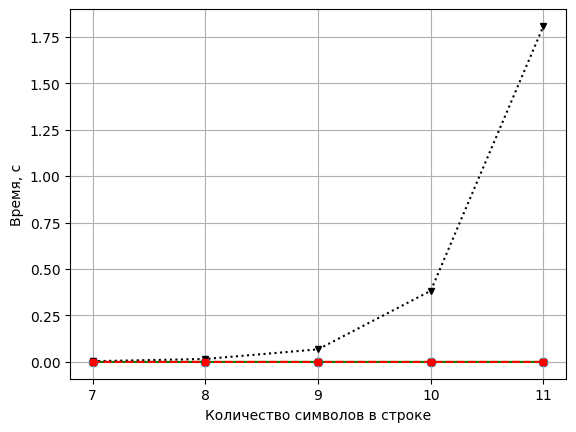
\includegraphics[scale=1]{График2.png}}
  \caption{Зависимость времени работы алгоритмов от длины строк}
  \label{img:algLevNRMatr, algDL3str, algLevRecNoCash}
\end{figure}
\newpage
Черная пунктирная кривая с треугольными маркерами -- 
алгоритм рекурсивного поиска расстояния Левенштейна 
без кэша; зеленая сплошная кривая с круглыми 
маркерами -- \\
нерекурсивный поиск расстояния 
Левенштейна с использованием матрицы; красная 
пунктирная кривая с квадратными маркерами -- поиск 
расстояния  Дамерау-Левенштейна с 
сохранением трех строк матрицы. На всех дальнейших 
графиках также используются данный обозначения.\\
Сравнение времени работы алгоритма на 7-ми 
символьных строках: \\
\begin{figure}[h]
  \center{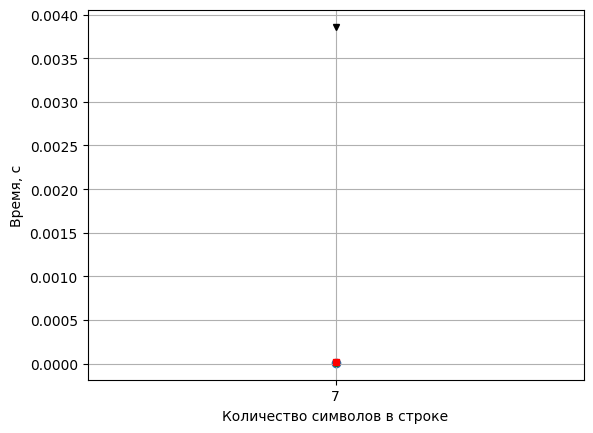
\includegraphics[scale=0.65]{График3.png}}
  \caption{Время работы со строкой длины 7}
  \label{img:algLevNRMatr, algDL3str, algLevRecNoCash}
\end{figure}
\begin{figure}[h]
  \center{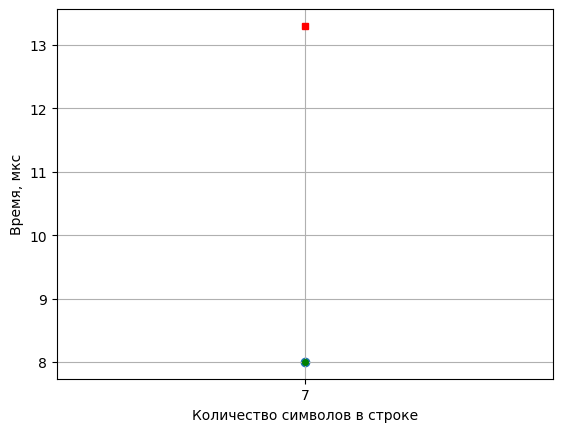
\includegraphics[scale=0.65]{График4.png}}
  \caption{Время работы со строкой длины 7}
  \label{img:algLevNRMatr and algDL3str}
\end{figure}\\
Такая большая разница в рекурсивном и нерекурсивном 
алгоритмах обусловлена тем, что во время 
рекурсии считаются одни и те же значения много 
раз (так как отсутствует кэш), при изменении длины 
строк, время будет расти экспоненциально. \\
Рассмотрим график для нерекурсивных реализаций:
\newpage
\begin{figure}[h]
  \center{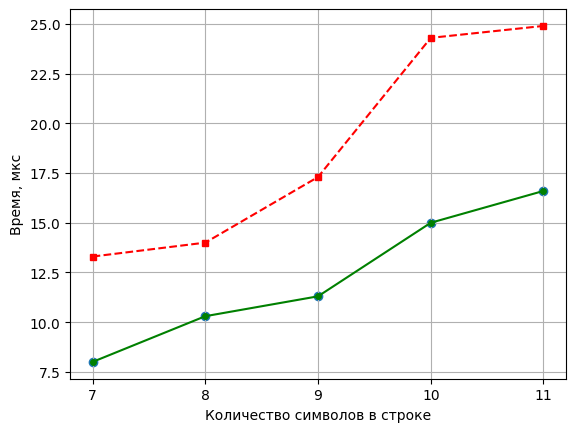
\includegraphics[scale=1]{График1.png}}
  \caption{Зависимость времени работы алгоритмов от длины строк}
  \label{img:algLevNRMatr and alg DL3str}
\end{figure}
Видно, что графики имеют похожий угол наклона, а изначальная 
разница во времени работы связана с тем, что при поиске
расстояния  Дамерау-Левенштейна хранятся только 3 строки, 
а значит время уходит на то, чтобы обновить эти строки для 
поиска следующей строки. Алгоритм рекурсивного поиска
расстояния Левенштейна без кэша хранит только строки и их
длины, затраты памяти увеличиваются экспоненциально, из-за 
чего использование его на больших строках оказывается 
невозможным.\\
Алгоритм нерекурсивного поиска расстояния Левенштейна с
использованием матрицы хранит всю матрицу, поэтому при 
увеличении длин строк, затраты памяти растут квадратично, что 
может затруднять работу с длинными строками. \\
Алгоритм поиска расстояния  Дамерау-Левенштейна с 
сохранением трех строк матрицы хранит только 3 строки матрицы 
и изначальные строки, а значит при увеличении длины 
изначальных строк, затраты памяти увеличиваются линейно.
\newpage

\section{Заключение}
В данной исследовательской работе было написано три алгоритма. 
По итогу сложно сказать, какой из всех реализованных 
алгоритмов оказался самым полезным и удобным на практике, но в
большинстве случаев борьба за первое место будет идти между 
двумя следующими алгоритмами: алгоритм поиска расстояния
Дамерау-Левенштейна с хранением трех строк матрицы и
алгоритм нерекурсивного поиска расстояния Левенштейна с
использованием матрицы. Время работы алгоритма поиска
расстояния Дамерау-Левенштейна с хранением трех строк
матрицы примерно в 1.5
раза больше времени работы алгоритма нерекурсивного поиска
расстояния Левенштейна с использованием матрицы (при
исследовании на строках длинны от 7 до 11), но все же
затраты времени одного порядка. При увеличении длины строк,
случае алгоритма Дамерау-Левенштейна с хранением трех 
строк матрицы, затраты памяти увеличиваются линейно, а не 
квадратично, как в алгоритме нерекурсивного поиска расстояния 
Левенштейна с использованием матрицы.
\newpage
\end{document}